\documentclass[border=1pt]{standalone}
\usepackage[dvipsnames]{xcolor}
\usepackage{tikz}                       % Graphen und kommutative Diagramme
\usetikzlibrary{patterns}               % Um schraffierte Formen in der tikzpicture-Umgebung zu zeichnen.
\newcommand{\ul}[1]{\underline{\smash{#1}}}

\begin{document}
\centering
\begin{minipage}{.4\textwidth}
\centering
\resizebox{!}{3.5cm}{
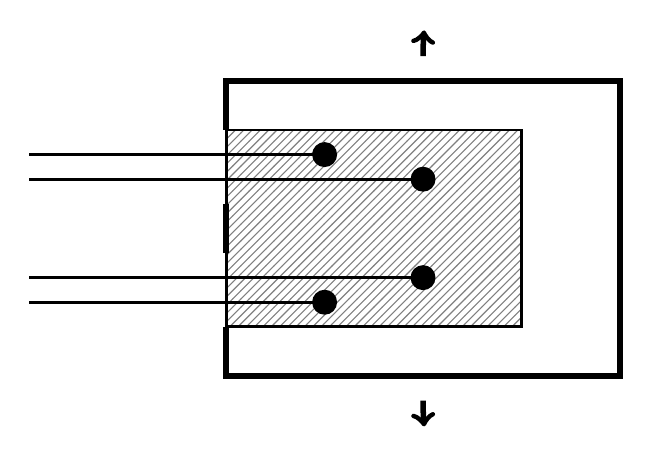
\begin{tikzpicture}[x=1.25cm, y=1.25cm, line width=1pt]
    % draw outer lines
    \draw (0, 0) -- (4, 0) -- (4, 3) -- (0, 3) -- (0, 0);
    
    % draw shaded slit box
    \filldraw[pattern=north east lines, pattern color=black!50] (0, 0.5) -- (3, 0.5) -- (3, 2.5) -- (0, 2.5) -- (0, 0.5);
    
    % draw line width=2pt boundary lines
    \draw[line width=2pt] (0, 0.5) -- (0, 0) -- (4, 0) -- (4, 3) -- (0, 3) -- (0, 2.5);
    \draw[line width=2pt] (0, 1.25) -- (0, 1.75);
        
    % draw slits
    \draw[color=black, line width=1.2pt] (-2, 1) -- (2, 1);
    \filldraw (2, 1)   circle (4pt);
    \draw[color=black, line width=1.2pt] (-2, 0.75) -- (1, 0.75);
    \filldraw (1, 0.75)   circle (4pt);
    \draw[color=black, line width=1.2pt] (-2, 2) -- (2, 2);
    \filldraw (2, 2)   circle (4pt);
    \draw[color=black, line width=1.2pt] (-2, 2.25) -- (1, 2.25);
    \filldraw (1, 2.25)   circle (4pt);
    
    % draw arrows
    \draw[->, line width = 2pt] (2, 3.25)  arc [radius = 3, start angle = 180, delta angle = -5];
    \draw[->, line width = 2pt] (2, -0.25) arc [radius = 3, start angle = 180, delta angle = 5];

\end{tikzpicture}
}
\end{minipage}

\centering
\begin{minipage}{.4\textwidth}
\centering
\resizebox{!}{4.5cm}{
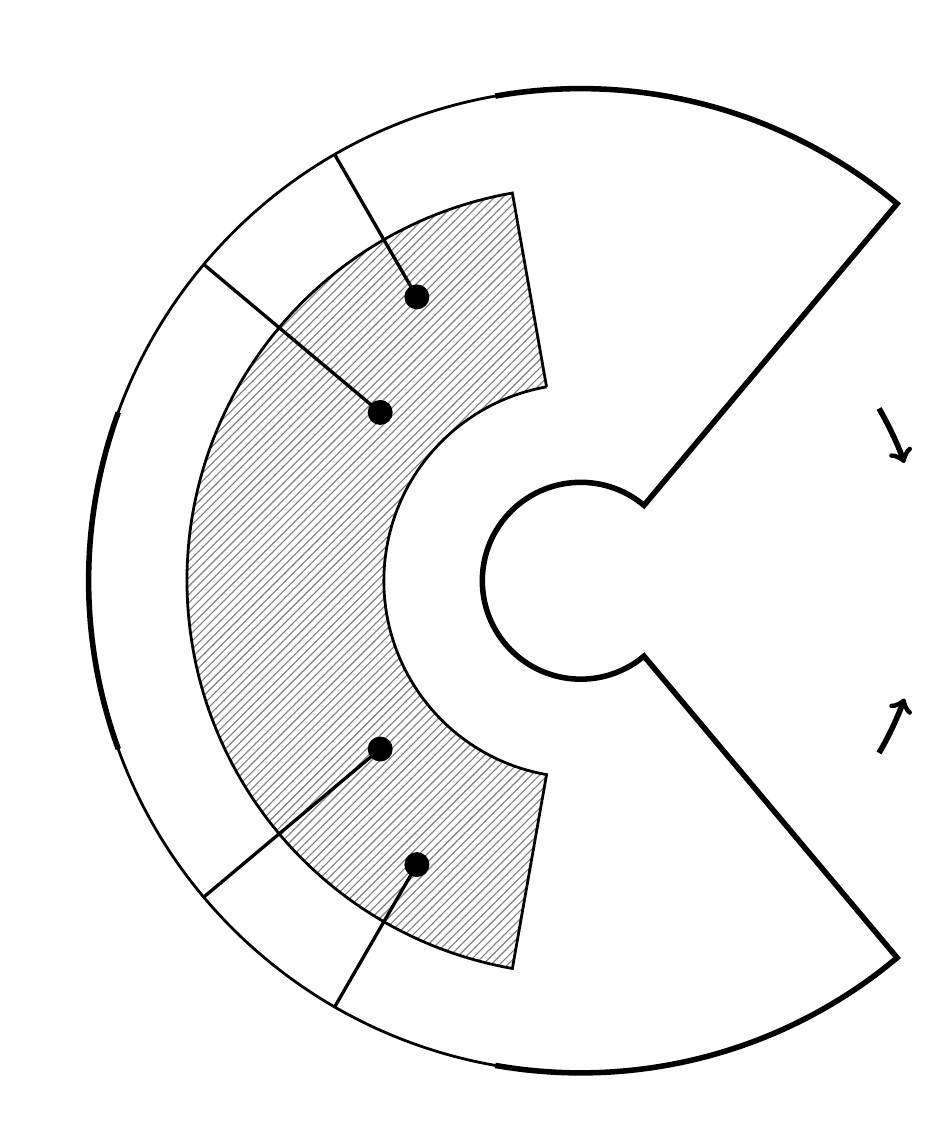
\begin{tikzpicture}[x=1.25cm, y=1.25cm, line width=1pt]
    % draw inner and outer circles
    \draw (50 : 1) -- (50 : 5)  arc [radius = 5, start angle = 50, delta angle = 260] 
	           -- (310 : 1) arc [radius = 1, start angle = 310, delta angle = -260] ;
    
    % draw shaded slit box
    \filldraw[pattern=north east lines, pattern color=black!50] 
       (100 : 2) -- (100: 4) arc [radius = 4, start angle = 100, delta angle = 160] 
 	         -- (260 : 2) arc [radius = 2, start angle = 260, delta angle = -160] ;
     
    % draw line width=2pt boundary lines
    \draw[line width=2pt] (100 : 5) arc [radius = 5, start angle = 100, delta angle = -50] -- (50 : 1)
	                   arc [radius = 1, start angle = 50, delta angle = 260] -- (310 : 5) 
	                   arc [radius = 5, start angle = 310, delta angle = -50];   
    \draw[line width=2pt] (160 : 5) arc [radius = 5, start angle = 160, delta angle = 40];

    % draw slits
    \draw[color=black, line width=1.2pt] (120 : 5) -- (120 : 3.33);
    \filldraw (120 : 3.33)   circle (4pt);
    \draw[color=black, line width=1.2pt] (140 : 5) -- (140 : 2.66);
    \filldraw (140 : 2.66)   circle (4pt);
    \draw[color=black, line width=1.2pt] (220 : 5) -- (220 : 2.66);
    \filldraw (220 : 2.66)   circle (4pt);
    \draw[color=black, line width=1.2pt] (240 : 5) -- (240 : 3.33);
    \filldraw (240 : 3.33)   circle (4pt);

    % draw arrows
    \draw[->, line width = 2pt] (30  : 3.5) arc [radius = 3.5, start angle = 30, delta angle = -10]; 
    \draw[->, line width = 2pt] (330 : 3.5) arc [radius = 3.5, start angle = 330, delta angle = 10]; 
     
\end{tikzpicture}
}
\end{minipage}

\centering
\begin{minipage}{.4\textwidth}
\centering
\resizebox{!}{4.5cm}{
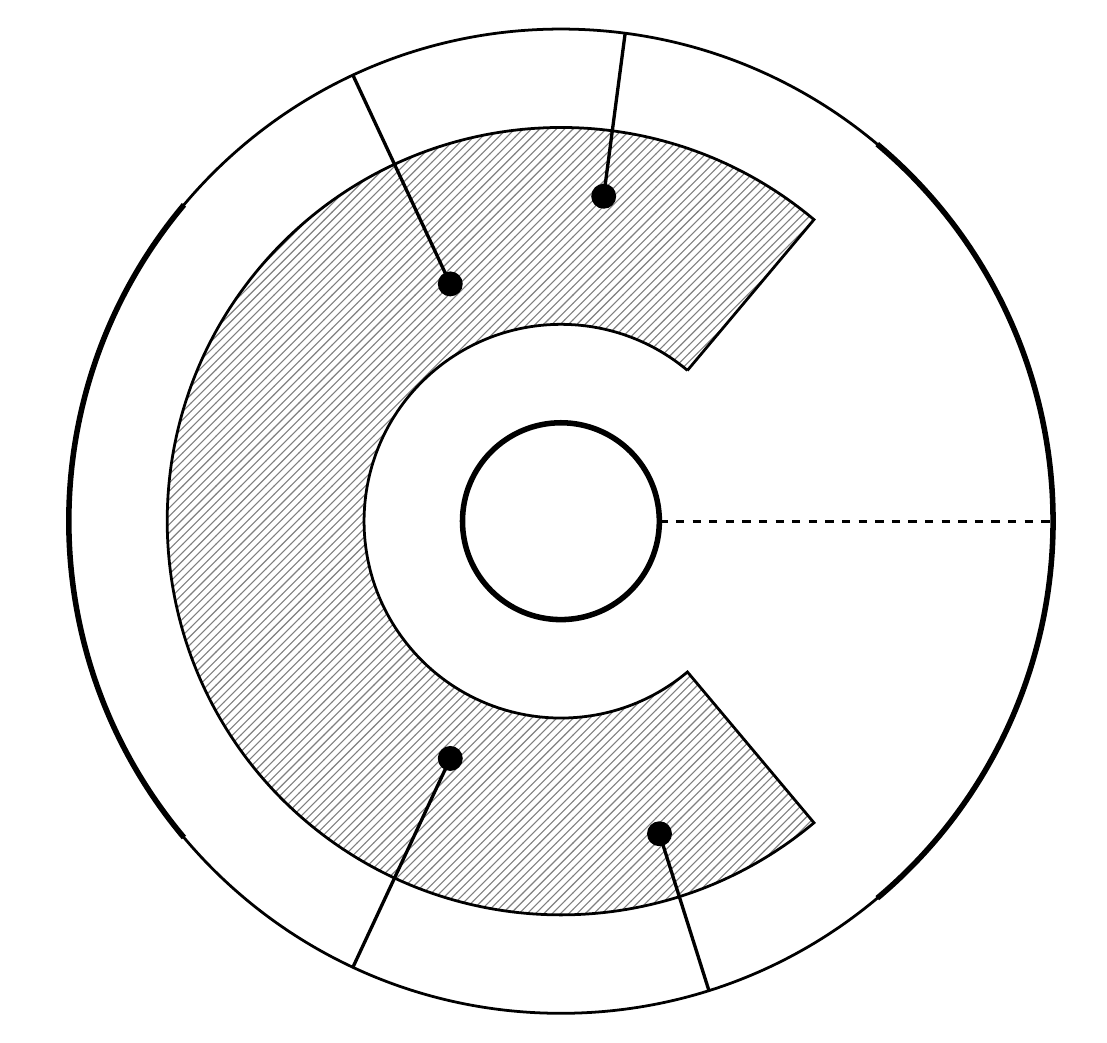
\begin{tikzpicture}[x=1.25cm, y=1.25cm, line width=1pt]
    % draw inner and outer circles
    \draw[color=black] (0, 0) circle (1);
    \draw[color=black] (0, 0) circle (5);
    
    % draw 0 line
    \draw[color=black, dashed] (0 : 1) -- (0 : 5); 
    
    % draw shaded slit box
    \filldraw[pattern=north east lines, pattern color=black!50] 
      (50 : 2) -- (50 : 4) arc [radius = 4, start angle = 50, delta angle = 260] 
	       -- (310 : 2) arc [radius = 2, start angle = 310, delta angle = -260] ;
    
    % draw line width=2pt boundary lines
    \draw[line width=2pt] (0 : 1) arc [radius = 1, start angle = 0, delta angle = 360]; 
    \draw[line width=2pt] (310 : 5) arc [radius = 5, start angle = 310, delta angle = 100]; 
    \draw[line width=2pt] (140 : 5) arc [radius = 5, start angle = 140, delta angle = 80]; 

    % draw slits
    \draw[color=black, line width=1.2pt] (82.5 : 5) -- (82.5 : 3.33);
    \filldraw (82.5 : 3.33)   circle (4pt);
    \draw[color=black, line width=1.2pt] (115 : 5) -- (115: 2.66);
    \filldraw (115 : 2.66)   circle (4pt);
    \draw[color=black, line width=1.2pt] (245 : 5) -- (245 : 2.66);
    \filldraw (245 : 2.66)   circle (4pt);
    \draw[color=black, line width=1.2pt] (287.5 : 5) -- (287.5 : 3.33);
    \filldraw (287.5 : 3.33)   circle (4pt);

\end{tikzpicture}
}
\end{minipage}


\end{document}
